\documentclass[12pt]{article}
\usepackage[utf8]{inputenc}
\usepackage[margin=1in]{geometry}
\usepackage{amsmath}\usepackage{amssymb}\usepackage{multicol}\usepackage{enumitem}
\usepackage{pgfplots}\pgfplotsset{compat=1.17}
\setlength{\parindent}{0pt}
\begin{document}

\fbox{\parbox{0.97\linewidth}{\small\textbf{Final answers} (record here --- graded on the answer; show your work):\\[6pt]1.~\underline{\hspace{1.5cm}}\quad 2.~\underline{\hspace{1.5cm}}\quad 3.~\underline{\hspace{1.5cm}}\quad 4.~\underline{\hspace{1.5cm}}\quad 5.~\underline{\hspace{1.5cm}}\quad 6.~\underline{\hspace{1.5cm}}\quad 7.~\underline{\hspace{1.5cm}}\quad 8.~\underline{\hspace{1.5cm}}\quad 9.~\underline{\hspace{1.5cm}}\quad 10.~\underline{\hspace{1.5cm}}\quad 11.~\underline{\hspace{1.5cm}}\quad 12.~\underline{\hspace{1.5cm}}}}
\vspace{0.35cm}

\begin{center}{\Large \textbf{Warm-Up: Vertex and Axis of Symmetry}}\end{center}\vspace{0.2cm}
% Warm-Up: Vertex and Axis of Symmetry
\textbf{Example (Warm-Up: Vertex and Axis of Symmetry):}

For $y=(x-4)^2+2$, vertex is $(4,2)$ and axis of symmetry is $x=4$.

\vspace{0.2cm}\hrule\vspace{0.35cm}
\textbf{Directions: State the vertex and axis of symmetry for each function.}

\begin{multicols}{2}
\begin{enumerate}[label=\textbf{\arabic*.}, start=1, itemsep=1.3cm]
  \item $\displaystyle y=(x-1)^2+3$
  \item $\displaystyle y=(x+2)^2-5$
  \item $\displaystyle y=2(x-3)^2+1$
  \item $\displaystyle y=-(x+4)^2+6$
\end{enumerate}
\end{multicols}
\vspace{0.25cm}\hrule\vspace{0.35cm}

\begin{center}{\Large \textbf{Find the y-intercept}}\end{center}\vspace{0.2cm}
% Find the y-intercept
\textbf{Example (Find the y-intercept):}

For $y=(x-2)^2+3$, substitute $x=0$: $y=(0-2)^2+3=7$, so the y-intercept is $(0,7)$.

\vspace{0.2cm}\hrule\vspace{0.35cm}
\textbf{Directions: Find the y-intercept for each function by substituting $x=0$.}

\begin{multicols}{2}
\begin{enumerate}[label=\textbf{\arabic*.}, start=5, itemsep=2cm]
  \item $\displaystyle y=(x-3)^2-1$
  \item $\displaystyle y=(x+1)^2+4$
  \item $\displaystyle y=2(x-1)^2-2$
  \item $\displaystyle y=-(x+3)^2+5$
\end{enumerate}
\end{multicols}
\vspace{0.25cm}\hrule\vspace{0.35cm}

\begin{center}{\Large \textbf{Full Graphs}}\end{center}\vspace{0.2cm}
% Full Graphs
\textbf{Example (Full Graphs):}

For $y=(x-1)^2-3$: vertex $(1,-3)$, axis $x=1$, y-intercept $(0,-2)$, mirror point $(2,-2)$. Plot and connect smoothly.

\begin{center}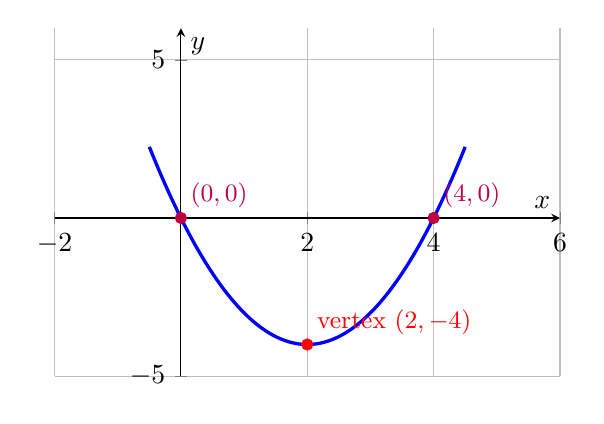
\begin{tikzpicture}
\begin{axis}[axis lines=middle,xlabel=$x$,ylabel=$y$,xmin=-2,xmax=6,ymin=-5,ymax=6,width=8cm,height=6cm,grid=both,samples=80]
\addplot[very thick,blue,domain=-0.5:4.5]{(x-2)^2-4};
\addplot[only marks,mark=*,red] coordinates {(2,-4)};
\node[above right,red,font=\small] at (axis cs:2,-4) {vertex $(2,-4)$};
\addplot[only marks,mark=*,purple] coordinates {(0,0)};
\node[above right,purple,font=\small] at (axis cs:0,0) {$(0,0)$};
\addplot[only marks,mark=*,purple] coordinates {(4,0)};
\node[above right,purple,font=\small] at (axis cs:4,0) {$(4,0)$};
\end{axis}\end{tikzpicture}\end{center}
{\small\centering Reference graph of $y=(x-2)^2-4$ showing the mirror-point technique.\par}
\vspace{0.2cm}\hrule\vspace{0.35cm}
\textbf{Directions: For each function, find the vertex, axis of symmetry, y-intercept, and its mirror point, then sketch the graph on the grid.}

\begin{multicols}{2}
\begin{enumerate}[label=\textbf{\arabic*.}, start=9, itemsep=3cm]
  \item $y=(x-2)^2-4$ (use the reference graph above to check your own sketch)
  \item $\displaystyle y=(x+2)^2-3$
  \item $\displaystyle y=2(x-1)^2+1$
\end{enumerate}
\end{multicols}

\vspace{0.2cm}\hrule\vspace{0.3cm}
\textbf{Challenge} (same sheet):\\[4pt]
\begin{enumerate}[label=\textbf{\arabic*.}, start=12, itemsep=2.2cm]
  \item Graph $y=-2(x-1)^2+3$ and label all key features (vertex, axis of symmetry, y-intercept, mirror point).
\end{enumerate}

\newpage

\begin{center}{\Large \textbf{Answer Key --- fully worked}}\end{center}
\vspace{0.25cm}
\textbf{Procedure:} Identify the vertex $(h,k)$ from the equation.; Draw the axis of symmetry as a dashed vertical line at $x=h$.; Find the y-intercept by substituting $x=0$ and solving for $y$.; Reflect the y-intercept across the axis of symmetry to get a mirror point.; Plot the vertex, y-intercept, and mirror point.; Connect the points with a smooth, U-shaped curve..\\[8pt]
\begin{enumerate}[label=\textbf{\arabic*.},itemsep=7pt]
  \item Vertex $(1,3)$; axis of symmetry $x=1$.
  \item Vertex $(-2,-5)$; axis of symmetry $x=-2$.
  \item Vertex $(3,1)$; axis of symmetry $x=3$.
  \item Vertex $(-4,6)$; axis of symmetry $x=-4$.
  \item $y=(0-3)^2-1=8$, so $(0,8)$.
  \item $y=(0+1)^2+4=5$, so $(0,5)$.
  \item $y=2(0-1)^2-2=0$, so $(0,0)$.
  \item $y=-(0+3)^2+5=-4$, so $(0,-4)$.
  \item Vertex $(2,-4)$, axis $x=2$, y-intercept $(0,0)$, mirror point $(4,0)$ -- matches the reference graph.
  \item Vertex $(-2,-3)$, axis $x=-2$, y-intercept: $y=(0+2)^2-3=1$, point $(0,1)$, mirror point $(-4,1)$.
  \item Vertex $(1,1)$, axis $x=1$, y-intercept: $y=2(0-1)^2+1=3$, point $(0,3)$, mirror point $(2,3)$.
  \item $y=-2(x-1)^2+3$: vertex $(1,3)$, axis of symmetry $x=1$, opens down (since $a=-2<0$). y-intercept: $y=-2(0-1)^2+3=-2+3=1$, point $(0,1)$; mirror point across $x=1$ is $(2,1)$. Plot $(1,3)$, $(0,1)$, $(2,1)$ and connect with a downward smooth curve.
\end{enumerate}

\end{document}